\chapter{Dagens situasjon} \label{chap:dagensSituasjon}
Dette kapittelet presenteres dagens situasjon knyttet til pasienters innsyn i informasjon om egen legemiddelbruk. Først presenteres legemiddelhåndteringsprosessen, og svakhetene ved den som gjør at pasienter kan ønske å ha innsyn i egen legemiddelsituasjon. Deretter presenteres hvilken rett pasienter har til innsyn i opplysninger lagret i egen journal, og hvordan pasienter kan få tilgang til disse opplysningene. Så presenteres kilder til legemiddelinformasjon som pasienter har tilgang til i dag, og pasientkontrollerte systemer som er er utviklet av store internasjonale selskaper, men som ikke er tatt i bruk i Norge. Til slutt presenteres lover og regler som skal sikte at personvernet er ivaretatt av personlige legemiddelinformasjonskilder.
 
\section{Legemiddelhåndteringsprosessen}
Dette delkapittelet beskriver de ulike aktivitetene som inngår i legemiddelhåndteringen, og informasjonsoverføringen som skjer mellom hver aktivitet. Legemiddelhåndtering beskriver legemiddelrelaterte oppgaver i en kjede av trinn fra legen beslutter bruk av et legemiddel til det er brukt av pasienten. I dette kapittelet er det valgt å dele inn legemiddelhåndteringsprosessen i følgende underaktiviteter: Ordinering, utlevering, dosering og inntak av dose, se figur~\ref{fig:prosess}.

\begin{figure}[h]
    \centering
    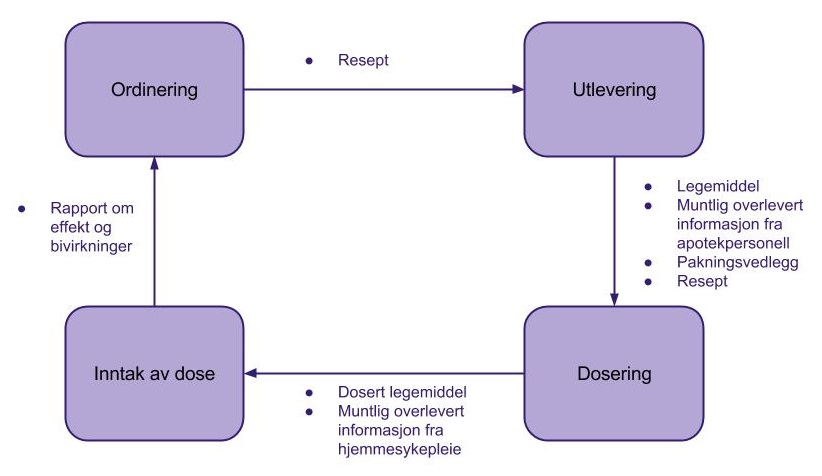
\includegraphics[width=0.9\textwidth]{fig/dagens/prosess.jpg}
    \caption{Aktivitetene ved legemiddelhåndtering og informasjonsoverføringen som finner sted mellom aktivitetene}
    \label{fig:prosess}
\end{figure}

\subsection{Ordinering}
Ordinering er at legen bestemmer bruk av legemiddel og dosering, og journalfører dette, jf. forskrift om legemiddelhåndtering § 3 bokstav g. Først har legen foretatt en medisinskfaglig vurdering, og funnet ut at pasienten trenger behandling med et eller flere legemidler. Legemidlene som ordineres er et ledd i en behandling hvor legen må passe på å angi riktig legemiddel og dosering. Legen skal kontrollere at ordineringen er forsvarlig med tanke på interaksjoner med andre legemidler i bruk, allergier og pasientens tilstand generelt. Legen skal skaffe oversikt over pasientens helsesituasjon gjennom direkte kontakt med pasienten og kommunikasjon med annet helsepersonell, jf. st. meld nr. 18 (2004-2005).
 
Etter en ordinering blir det gjort en rekvirering. Rekvirering er definert som en “muntlig, skriftlig eller elektronisk bestilling av legemiddel ved resept eller rekvisisjon”, jf. forskrift om legemidler fra apotek § 1-3 bokstav e og forskrift om legemiddelhåndtering § 3 bokstav f. Det vanligste er at bestillingen blir opprettet som en elektronisk resept (eResept). Bestillingen som opprettes ved rekvirering er en del av informasjonsutvekslingen fra ordineringsfasen til utleveringsfasen.
 
Ifølge helsepersonelloven § 11 kan leger rekvirere reseptbelagte legemidler. De fleste rekvireringer av legemidler gjøres av fastlegen, men mange rekvireringer skjer også av leger i spesialisthelsetjenesten \citep{stmeld1820042005}.Det at flere leger rekvirerer legemidler til den samme pasienten kan gjøre det vanskelig for legene å holde oversikt over hvilke legemidler pasienten står på. 

Fastlegeordningen ble innført i Norge i 2001, og skal sikre at alle som ønsker det har én bestemt allmennlege å forholde seg til. I følge forskrift om fastlegeordning i kommunene § 10 er en fastlege i utgangspunktet ansvarlig for å tilby alle typer “allmennlegeoppgaver” for innbyggerne på sin liste.  Det er vanskelig å avgjøre hva som er “allmennlegeoppgaver” da ordlyden er vid og uklar. Dette gjør at det er vanskelig å avklare nøyaktig hva som er fastlegens ansvar knyttet til sine pasienters legemiddelbruk. 

Forskrift om fastlegeordning i kommunene § 25 kan bidra til å få klarhet i dette. Ifølge forskriften skal fastlegen “koordinere” legemiddelbehandlingen til innbyggerne på sin liste. Dette innebærer å oppdatere legemiddellisten til pasienten når fastlegen endrer eller får informasjon om at legemiddelbehandlingen er endret. For at fastlegen skal kunne oppdatere legemiddellisten er det altså viktig at informasjon om endringer av andre blir formidlet til fastlegen. Pasienter har ofte feil legemiddellister på grunn av dårlig informasjonsutveksling mellom ulike aktører eller fordi informasjon som blir utvekslet ikke blir fulgt opp. Sykehusepikrisen fungerer ofte som eneste form for informasjonsoverføring fra spesialisthelsetjenesten til fastlegene. En undersøkelse gjort i Tromsø \citep{komLegemidler} i 2007 viste at mange epikriser kom frem svært sent (noen ganger ble ikke epikrisen sendt ut i det hele tatt) og det var bare tre av ni leger som oppdaterte legemiddellisten når de mottok epikrise fra sykehusene.

Det følger av forskrift om fastlegeordning i kommunene § 14 at dersom en person som står på fastlegens liste blir inntatt i en helse- og omsorgsinstitusjon eller annen institusjon med organisert legetjeneste, overføres legemiddellisteansvaret etter forskriftens § 10 til institusjonen. Mens pasienten er på institusjon har altså ikke fastlegen lenger ansvar fordi institusjonen overtar det ansvaret fastlegen tidligere hadde. For å kunne overta ansvaret på en god måte trenger institusjonen informasjon fra fastlegen om pasientens legemiddelliste. Det er ikke alltid denne informasjonsoverføringen fungerer optimalt. Særlig legevakten har hatt problemer med at de ikke mottar nødvendige opplysninger om legemiddelbruk \citep{komLegemidler}. 

\subsection{Legemiddelgjennomgang} \label{subsec:legemiddelgjennomgang} 
Legemidler brukes ofte ikke slik de er tiltenkt, noe som kan føre til legemiddelrelaterte problemer\footnote{Legemiddelrelatert problem: “en hendelse eller et forhold som skjer i forbindelse med legemiddelbehandling og som reelt eller potensielt interfererer med ønsket helseeffekt”\citep{legemiddelgjennomgang}} \citep{WHO}. Mange av disse problemene kan enkelt forebygges. Et av tiltakene som er iverksatt for å begrense og forebygge legemiddelrelaterte problemer er at leger skal gjennomføre legemiddelgjennomgang av pasientenes legemidler. 

En legemiddelgjennomgang er en “strukturert/systematisk evaluering av den enkelte pasientens legemiddelregime i den hensikt å optimalisere effekten av legemidlene og redusere risiko ved legemiddelbruk” \citep{legemiddelgjennomgang}. En legemiddelgjennomgang kan resultere i at at pasientens legemiddelliste endres.

Legemiddelgjennomgang kan gjøres av behandlende lege alene eller sammen med sykepleiere, farmasøyter eller pasienten det gjelder. Behandlende lege er ansvarlig for beslutninger fattet i forbindelse med legemiddelbehandling av pasienter. Derfor er behandlende lege ansvarlig for de endelige beslutningene tatt i legemiddelgjennomgangen.

Før det kan gjøres en legemiddelgjennomgang må det gjøres en legemiddelsamstemming. En legemiddelsamstemming vil si at det lages en korrekt liste over alle legemidlene en pasient bruker. Listen som utarbeides i samstemmingsprosessen kalles “Legemidler i bruk” (\acrshort{lib}). Informasjonen som trengs for å lage listen hentes blant annet fra e-resepter, pasientjournaler og pasientens egen liste \citep{sjekklisteLegemiddelgjennomgang}.
 
En legemiddelgjennomgang skal utføres ved endring i situasjon, eller regelmessig dersom pasienten tar minst fire legemidler, jf. Forskrift om fastlegeordning i kommunene § 25. I følge forskriften er det fastlegen som er ansvarlig for at en slik legemiddelgjennomgang blir gjennomført.
 
Legemiddelverket har lansert en sjekkliste\footnote{Les mer om legemiddelverkets sjekkliste for legemiddelgjennomgang her:\url{http://www.kunnskapssenteret.no/verktoy/sjekkliste-for-legemiddelgjennomgang}} for legemiddelgjennomgang. Det er en kortfattet veiledning som inneholder sjekkpunkter og en liste med legemidler man bør være spesielt oppmerksomme på. Sjekklisten bygger blant annet på \acrshort{start}/\acrshort{stopp}-kriteriene og \acrshort{norgep}. Mer om legemiddelgjennomgang i delkapittel~\ref{sec:littLegemiddelgjennomgang}.

\subsubsection{Start Stopp NorGeP}
De fleste legemidler har bivirkninger, og det er derfor ønskelig at pasienter ikke tar flere legemidler enn nødvendig. Det er derfor publisert tre verktøy som skal hjelpe legen med å vurdere om alle pasientens legemidler er nødvendige, og om pasienten får alle nødvendige legemidler. De tre verktøyene heter: \acrshort{start}, \acrshort{stopp} og \acrshort{norgep}. 

\acrshort{start} og \acrshort{stopp} er utviklet i Irland. De har blitt oversatt til norsk med noen justeringer for at de skal samsvare med norsk terapitradisjon. I 2015 ble \acrshort{start} og \acrshort{stopp} oppdatert med ny informasjon. De nye versjonene heter START2 og STOPP2. \acrshort{norgep} er utviklet i Norge. 

\acrshort{start}, \acrshort{stopp} og \acrshort{norgep} har særlig fokus på eldre. Mange eldre mennesker får legemidler for flere lidelser, og er spesielt utsatt for uheldige effekter av legemiddelbehandling. Forandringer som skjer i kroppen grunnet høy alder gjøre at farmodynamikken endrer seg.

\acrshort{start}\footnote{Les mer om START her: \url{http://legemiddelhandboka.no/Generelle/311103}}(\acrlong{start}) er et hjelpemiddel for å sjekke at pasienter får de anbefalte legemidlene ved lidelser som ofte ikke behandles tilstrekkelig hos eldre.
 
\acrshort{stopp}\footnote{Les mer om STOPP her: \url{http://legemiddelhandboka.no/Generelle/315753}}(\acrlong{stopp}) er et hjelpemiddel som skal synliggjøre potensielle uhensiktsmessige legemidler. Stopp er egnet for både allmennpraksis og sykehus.

\acrshort{norgep}\footnote{Les mer om NorGeP her: \url{http://legemiddelhandboka.no/Generelle/311393}}(\acrlong{norgep}) inneholder en relevant liste av legemidler, legemiddeldoser, og legemiddelkombinasjoner som bør unngås av eldre over 70 år. 

\subsubsection{Resept}
Resept er definert som en bestilling av et legemiddel, jf. forskrift om legemidler fra apotek §1-3 bokstav c. En repsept er er en del av informasjonsflyten fra ordineringsfasen til utleveringsfasen. Fra og med tidlig 2013 er de fleste resepter i Norge elektroniske. Det finnes ulike typer resepter. Forskjellen mellom disse er forklart i de to neste avsnittene.

Legemidler som er klassifisert som sterke narkotiske stoffer må rekvireres på en spesialblankett som kalles narkotikaresept eller A-resept. Hvis legemiddelet som rekvireres er klassifisert som et vanedannende legemiddel omtales resepten gjerne som B-resept. C-resept er for alle reseptpliktige legemidler som ikke omfattes av A- eller B-resept.

Blå resept skrives ut når pasienten har krav på å få dekket deler av legemiddelutgiftene av staten. For legemidler rekvirert på hvit resept må utgifter dekkes av pasienten. 

\subsection{Utlevering}
I Norge har apotekene enerett til å selge og utlevere legemidler, jf. legemiddelloven § 16 andre ledd. Forarbeidene\footnote{Ot.prp. nr. 29 (1998-99)} forklarer at denne eneretten skal bidra til å sikre at legemidlene har god kvalitet og at de blir riktig oppbevart. Apotekene har leveringsplikt for alle legemidler, og skal sørge for at legemidler og viktig medisinsk utstyr er tilgjengelig \citep{apotekOgLegemidler2013}.
 
Apotekene er kompetansebedrifter som skal bidra til riktig og rasjonell legemiddelbruk. De skal hindre feilbruk og uheldig overforbruk av legemidler gjennom veiledning og farmasøytiske tjeneste. Det følger av forskrift\footnote{Forskrift om legemidler fra apotek § 8-2}, at apotekene skal bidra til at den som mottar legemidler har “tilstrekkelige” opplysninger om legemidlet til at det kan brukes riktig.

På apotek jobber farmasøyter og apotekteknikere. Titlene farmasøyt og apotekteknikker kan bare benyttes i Norge om personer som er autorisert etter helsepersonelloven. Farmasøyter som jobber på apotek har ansvar for å utlevere legemidlene til pasienten, kontrollere resepten og veilede om bruk. Apotekteknikerne har kontakt med kundene på apoteket og bistår farmasøytene.
 
Tradisjonelt har farmasøytrollen bare vært knyttet til legemiddelet som produkt, og ekspedering av legemidler. Det fokuseres nå også på oppgaven å gi informasjon om riktig legemiddelbruk, samt bidra til å avdekke og forebygge legemiddelrelaterte problemer. Det er imidlertid ikke helt klart hvor langt denne oppgaven strekker seg, og hva apotekets informasjonsplikt innebærer. Helse og omsorgsdepartementet påpeker i forarbeidene til apotekloven\footnote{Ot.prp. nr. 29 (1998-99)} at ansvaret for legemiddelinformasjon knyttet til behandling alltid påhviler legen. Det er derfor viktig at apoteket ikke gir informasjon som strider mot det legen har bestemt. For legemidler som ikke er reseptpliktige stiller saken seg annerledes. I disse tilfellene har det ikke vært noen lege som har vurdert legemiddelbehovet. Dermed får apoteket et hovedansvar for at kunden får tilstrekkelig informasjon. For legemidler uten resept kan apoteket komme i en situasjon hvor de må gi råd om ikke-bruk eller ikke-salg.

\subsubsection{Sykehusapotekene}
Det er 30 sykehusapotek i Norge. I apotekloven §1-3 bokstav d er et sykehusapotek definer som et “apotek i samlokalisering med offentlig sykehus eller privat sykehus som inngår i offentlige helseplaner, som har legemiddelforsyning til sykehuset som sin primæroppgave”. 

Staten overtok eieransvaret for de offentlige sykehusene ved sykehusreformen som ble innført i 2002. Som følge av sykehusreformen ble sykehusapotekene en del av spesialisthelsetjenesten, de ble overført til staten og videre til de regionale helseforetakene (Helse Sør-Øst, Helse Vest, Helse Midt-Norge, Helse Nord). 

Formålet med sykehusapotekene er fastsatt av det regionale helseforetaket de tilhører, og skiller seg derfor noe fra region til region. Felles for alle sykehusapotek er at de skal sikre forsyningen av legemidler til det sykehuset apoteket er tilknyttet, være pasientenes og sykehusets kompetansesenter for legemidler og produsere de legemidler som ikke kan skaffes på annen måte, så langt det lar seg gjøre \citep{sykehusapotekenesOrganisering}. 

\subsection{Dosering}
I forskrift om legemiddelhåndtering § 3 bokstav d defineres istandgjøring av legemidler som ”Tilberedning eller annen klargjøring av legemiddel for utdeling til pasient.”. Utdeling av legemidler skjer på ulike måter avhengig av hvor pasienten er og hvilke tjenester pasienten benytter seg av. I merknadene til forskriften\footnote{Merknader til forskrift om legemiddelhåndtering for virksomheter og helsepersonell som yter helsehjelp, Til §2} står det at det ved avtale eller vedtak kan bestemmes at hjemmesykepleien har ansvaret for istandgjøring av en pasients legemidler. 

For de som bruker flere legemidler er det viktig å holde legemidler for hvert inntakstidspunkt atskilt. Ved bruk av multidose\footnote{Multidose: maskinpakket, forseglet pose som inneholder legemidlene pasienten skal ta til et bestemt tidspunkt på dagen.} kommer legemidlene ferdig pakket og merket med inntakstidspunkt. Et annet hjelpemiddel som også brukes av hjemmesykepleien for å dosere pasientenes legemidler er dosett \citep{HelsetilsynetRapport}. 

På institusjon og i hjemmesykepleien har sykepleiere eller vernepleiere ansvar for at legens ordinasjon blir fulgt. Det vil si å sørge for at rett legemiddel gis til rett pasient, i rett legemiddelform, i rett dose, på rett måte, til rett tid og med rett informasjon. Oppgaven er en delegert legeoppgave, jf. Helsepersonelloven § 5. Oppgaven innebærer også at sykepleieren har ansvar for å foreta observasjon av behandlingens effekt, og gi lege beskjed dersom noe uventet inntreffer \citep{IllustrertFarmakologi}. 

Dersom legemidlene er dosert og satt frem av én person, men gis til pasienten av en annen, er det den som gir legemidlet til pasienten som er ansvarlig for at alt er korrekt. Det er derfor viktig at den som deler ut legemiddelet sjekker at legens ordinering er fulgt \citep{IllustrertFarmakologi}. 

For at sykepleiere/vernepleiere skal kunne gi riktige legemidler er det viktig at de har tilgang til korrekt informasjon om hva legen har bestemt. I en studie i Tromsø \citep{komLegemidler} kom det frem at særlig hjemmetjenesten ikke var fornøyd med tilgangen til og kvaliteten på informasjonen om medisinering. I undersøkelsen kom det frem at resept ofte fungerte som eneste skriftlige kommunikasjon fra fastlegen til hjemmesykepleien. 

Pasienter som befinner seg utenfor helseinstitusjoner, og ikke benytter seg av hjemmesykepleie, har selv ansvar for at legemidlene tas etter legens anvisning. Legen og apoteket har et ansvar om å gi tilstrekkelig informasjon til at pasienten kan ta legemidlene riktig. 

\subsubsection{Dosett}
Dosett er en oppbevaringsbeholder for tabletter eller kapsler. Figur~\ref{fig:dosett} viser hvordan en dosett kan se ut. I en dosett sorteres legemidlene etter mengde og inntakstid. Meningen med dosett er å forenkle dosering av legemidler.

\begin{figure}[h]
    \centering
    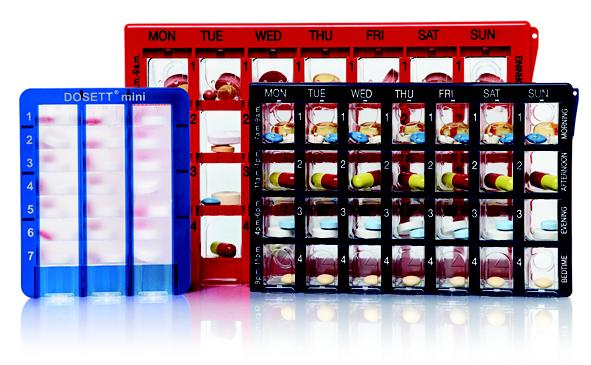
\includegraphics[width=0.6\textwidth]{fig/dagens/dosett.jpg}
    \caption{Ulike typer dosett, hentet fra: \url{http://www.dosett.com/}}
    \label{fig:dosett}
\end{figure}

\subsubsection{Multidose}
Multidose er en maskinpakket, forseglet pose som inneholder legemidlene pasienten skal ta til et bestemt tidspunkt på dagen, se Figur~\ref{fig:multidose}. Multidose er ment å være et virkemiddel for å sikre riktig legemiddelhåndtering, og forenkle hverdagen for brukere med flere medikamenter, pårørende og helsetjenesteytere \citep{OmMultidose}. Multidose brukes av pasienter med stabil legemiddelbruk, slik at legemiddellisten ikke endres fra multidosen er bestilt til alle legemidlene i multidoserullen er inntatt. 

\begin{figure}[h]
\centering
\makebox[\linewidth][c]{%
\begin{subfigure}[b]{2in}
    \centering
	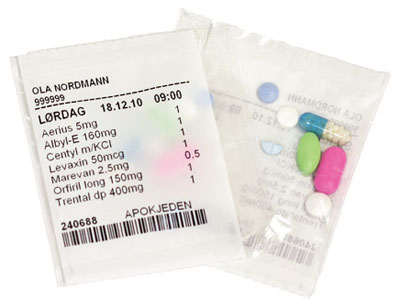
\includegraphics[width=2in]{fig/dagens/dosepakking.jpg}
	\caption{Multidosepakke}\label{fig:multidosepakke}
\end{subfigure}
\quad
\begin{subfigure}[b]{3.2in}
    \centering
    
\includegraphics[width=3.2in]{fig/dagens/multidoserull.jpg}
    \caption{Multidoserull}\label{fig:multidoserull}
\end{subfigure}
}
\caption{Bilder av multidosepakninger, hentet fra: \url{http://www.apotek1.no/multidose/faa-legemidlene-dine-pakket-i-ferdige-doser}}\label{fig:multidose}
\end{figure}

Pasienter med multidose har mindre kunnskap om legemidlene de tar enn andre pasienter \citep{Kwint01092013}. På multidosepakningene finnes det kun informasjon om legemidlets navn og inntaks tidspunk, det står ikke noe om hva medisinen skal behandle. På multidosepakningen er det altså en meget begrenset mengde informasjon om legemidlene som er tilgjengelig. I tillegg står informasjonen på multidosepakkene med liten skrift, noe som gir redusert lesbarhet for brukere med dårlig syn. 

Innføring av multidose har gitt høyere etterlevelse, og ført til at legemiddellistene er bedre samenstilt mellom ulike instanser \citep{Wekre01102010}. Legemiddellistene til pasienter med multidose blir imidlertid sjeldnere revidert enn pasienter som får tradisjonell forskrivning \citep{mutiDose,Larsen2007265}. Leger opplever at justeringer av legemidler/doser er mer krevende når pasienter bruker multidose \citep{doi:10.3109/02813432.2011.554002}, og leger har ulik oppfatning om hvem som som har ansvaret for legemiddellisten til pasienter som flere leger kan rekvirere multidose til \citep{Rahmner01012010, Wekre01082012}.

Studier har vist at pasienter på multidose oftere har en uhensiktsmessig legemiddelliste, med flere potensielt farlige kombinasjoner av legemidler, enn pasienter som får vanlig ordinering \citep{23295105, PDS:PDS2232}. Det er beregnet at pasienter med multidose har 5,9 ganger høyere sjanse enn andre for å bli utsatt for feil i forbindelse med legemidler \citep{multidoseFeil}. Denne beregningen kan delvis skyldes at det er lettere å oppdage problemer hos pasienter med multidose. Multidosepakningen gir en oversikt over hvilke legemidler pasienten tar, noe som kan gjøre det lettere å se hvilke feil som eksisterer.

\subsection{Inntak av dose}
Siste aktivitet i legemiddelhåndteringen er at pasienten inntar legemiddelet.

Hjemmesykepleien eller annet pleiepersonell hjelper ofte til med å gjøre i stand dosen som skal tas. De kan klargjøre en dosett (for en hel uke), som pasienten selv må ta riktige legemidler fra, eller de kan ha klargjøre den enkelte dosen. Det er vanlig at pasienten inntar legemiddelet selv \citep{AutomatiskPilledispenser}.
 
Noen pasienter får hjelp til å innta noen typer legemidler. Det er for eksempel vanlig å få hjelp til å ta sprøyter. Dersom pasienten har kraftige funksjonshemninger kan pasienten få hjelp med inntak av legemidler på former som ellers er vanlig å ta selv. For eksempel kan en pasient som ikke har bevegelse i armene få hjelp med å føre en tablett til munnen. 

\subsubsection{Oppfølging av medisineringens effekt}
I følge \citep{HelsetilsynetRapport} foreligger det ingen retningslinjer på hvordan effekt av medisinering skal registreres, observeres og følges opp. I hjemmesykepleien er det vanlig at avdelingssykepleieren instruerer resten av personalet i hva som bør følges ekstra med på hos den enkelte pasient. Pleiepersonalet rapporterer uvanlige reaksjoner på legemidler. I hjemmesykepleien og på sykehjem blir dette ført inn i den elektroniske journalen for hver enkelt pasient. Denne journalen brukes primært av vakthavende sykepleier, og blir ikke lest på rutinebasis av legen på sykehjemmet. Fastlegen har ikke direkte tilgang til journalen til hjemmesykepleien.

\subsection{Oppsummering av legemiddelhåndteringsprosessen}
Legemiddelhåndtering er en prosesss som involverer mange aktører. Siden mange deltar i arbeidet kan det være vanskelig for den enkelte å holde oversikt over hele prosessen. Fordi det er mange prosessledd involvert i legemiddelhåndteringen er det viktig at informasjonsoverføringen mellom leddene er god, for å sikre at aktørene har tilgang på korrekt og fullstendig informasjon. Mange legemiddelskader skjer på grunn av dårlig informasjonsoverføring \citep{HelsetilsynetRapport, komLegemidler}.

Helsetilsynet beskriver legemiddelhåndteringsprosessen på følgende måte:
“Prosessen kjennetegnes av at den gjennomføres av personell som ser lite til hverandre i det daglige arbeidet, som for eksempel lege, apotek og pleiepersonale. Dette gjør den ekstra sårbar for misforståelser og feil, særlig når informasjon overføres fra et prosessledd til det neste.” \citep{HelsetilsynetRapport} 

Lover og forskrifter er uklar på hvilke aktører som har ansvar for hva, og hvor langt de ulike aktørenes ansvar strekker seg. Dette gjør det vanskelig for hver aktør å vite om de tar ansvar for det de skal, og når de beveger seg ut på andres ansvarsområde. 

Når det skjer feil i legemiddelhåndteringsprosessen som gjør at pasienten får dårligere legemiddelbehandling er det pasienten som blir skadelidende. Det kan derfor være nyttig for pasienten å ha innsikt i egen legemiddelsituasjon. 


\section{Rett til innsyn}
Norsk lovgivning gir pasienter rett til innsyn i egen journal, jf. helsepersonelloven § 41, helseregisterloven kapittel 4, personopplysningsloven kapittel 3 og pasient- og brukerrettighetsloven kapittel 5. Innsyn i egne helseopplysninger gir innblikk i hvilke opplysninger som er registrert, hvordan opplysningene brukes og hvem som har tilgang til opplysningene. Innsyn i egen journal kan gi pasienten økt innsikt i og kontroll over egen helsesituasjon.

Dagens løsninger for innsyn i egen journal er imidlertid tungvinte. Informasjonsteknologi gir muligheter for enklere tilgang til egne helseopplysninger. I følge stortingsmelding 9 (2012–2013) “Én innbygger – én journal” gir informasjonsteknologi grunnlag for mer delaktighet og en demokratisering av pasientens rolle. Stortingsmeldingen har følgende mål:

\begin{itemize}
 \item Helseopplysninger skal følge pasienter gjennom hele pasientforløpet.
 \item Pasienter skal ha elektronisk tilgang til egen journal.
 \item Pasienter og helsepersonell skal kunne kommunisere elektronisk med hverandre.
 \item Selvbetjeningsløsninger skal være tilgjengelige for pasienter.
 \item Informasjon om helse- og omsorgstjenesten skal være tilgjengelig for pasienter
\end{itemize}

\section{Kilder til informasjon}
Her presenteres kilder tilgjengelig for pasienter i Norge i dag. Det inkluderer både kilder til personlig informasjon om hver enkelt pasient sine legemidler, og kilder til informasjon om alle legemidler som er markedsført i Norge. 

\subsection{Helsedirektoratet}
Helsedirektoratet er et fagdirektorat og et myndighetsorgan. Helsedirektoratet blir etatstyrt av helse og omsorgsdepartementet. Helsedirektoratet er ansvarlig for flere tjenester som gir folk innsyn i informasjon om deres egen helse, blant annet \url{https://helsenorge.no/}. 

\subsection{Pakningsvedlegg}
Alle legemidler som blir markedsført i Norge skal ha et pakningsvedlegg med informasjon om preparatet, jf. legemiddelforskriften § 3-42. I pakningsvedlegget finnes informasjon om mulige bivirkninger, virkemåte, forsiktighetsregler og dosering.

Helsedirektoratet anbefaler å lese pakningsvedlegget som en bruksanvisning til medikamentene. Pakningsvedlegget inneholder svært mye informasjon og kan være vanskelig å få oversikt over. 

\subsection{Helsenorge.no}
Helsenorge.no er en portal som er ment å være den nasjonale inngangsporten til helse- og omsorgstjenester på nett. Alle i Norge med personnummer eller D-nummer, samt elektronisk ID på høyeste sikkerhetsnivå\footnote{Les mer om de ulike sikkerhetsnivåene her: \url{http://eid.difi.no/nb/sikkerhet-og-personvern/informasjon-om-sikkerhetsniva}}, har tilgang til denne tjenesten. 

På portalen finnes informasjon om sykdom og behandling, samt enkelte tjenester for innsyn i egne data og løsninger for selvbetjening. Eksempler på tjenester man kan finne på helsenorge.no er “Mine resepter”, “finne eller bytte fastlege”, “Mine egenandeler”, “Mine vaksiner” og “Kjernejournal”.

\subsection{Mine resepter}
For å holde oversikt over aktive resepter tilbyr Helsedirektoratet en internettbasert tjeneste\footnote{Mine resepter finner du på: \url{https://www.mineresepter.no/}}. Alle som har fått en eller flere elektroniske resepter kan benytte tjenesten. Siden har oversikt over aktive resepter, legemidler som har blitt utlevert og hvor mange utleveringer som gjenstår. Figur~\ref{fig:mineResepter} viser et skjermbilde fra \url{www.mineresepter.no}.

\begin{figure}[H]
  \centering
    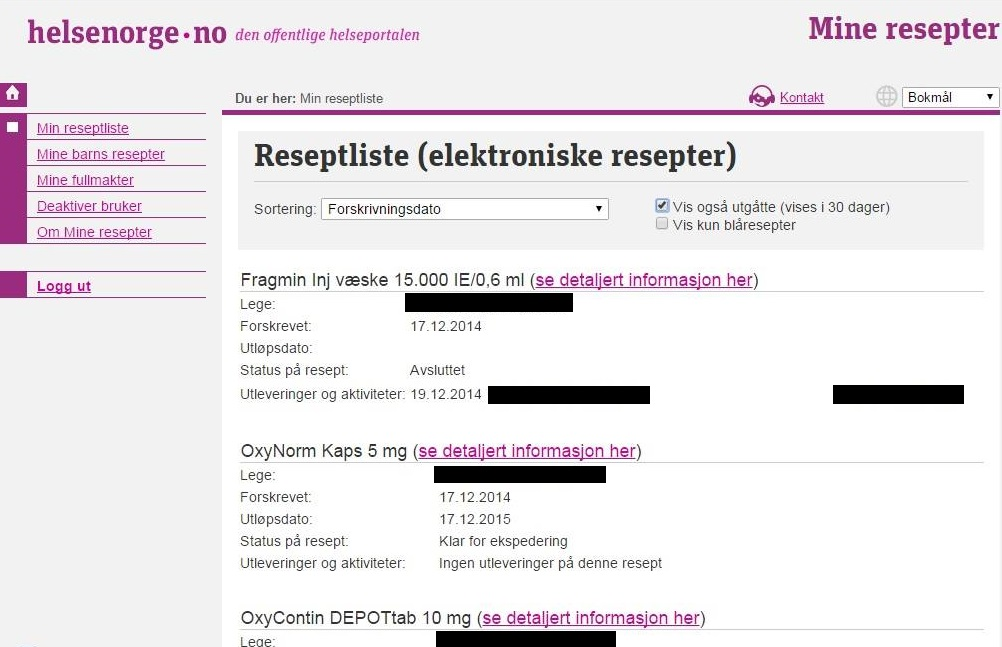
\includegraphics[width=1\textwidth]{fig/dagens/mineresepter.jpg}
  \caption{Skjermbilde som viser hvordan en reseptliste kan se ut på \url{www.minereseper.no}. Dato:19.12.2014}
\label{fig:mineResepter}
\end{figure}

\begin{figure}[H]
  \centering
    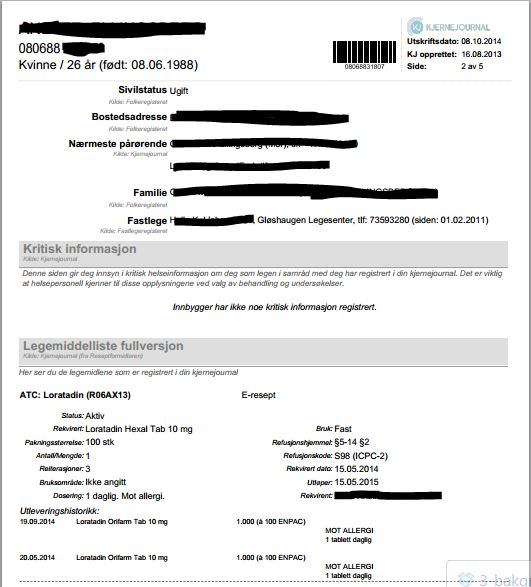
\includegraphics[width=1\textwidth]{fig/dagens/kjernejournal2.jpg}
  \caption{Skjermbilde som viser eksempel på en kjernejournal. Dato: 08.10.2014}
\label{fig:kjernejournal}
\end{figure}

\subsection{Kjernejournal}
Innbyggere i noen kommuner har tilgang til kjernejournal via helsenorge.no. Kjernejournal er et prøveprosjekt i enkelte kommuner i landet, med mål om å samle helseopplysninger på ett sted. Ved ulykke i utlandet kan det være betryggende for den utsatte å ha tilgang til egne helseopplysninger uten å være avhengig av samordning på tvers av landegrenser.

Kjernejournal er et supplement til journaler som føres hos lege eller på sykehus, og inneholder helseopplysninger som kan være viktige for helsepersonell å vite om, spesielt i akutte situasjoner. Opplysningene hentes automatisk fra offentlige register, blant annet personalia (fra Folkeregisteret), fastlege (fra Fastlegeregisteret), legemidler utlevert på resept i norske apotek (Reseptformidleren\footnote{Reseptformidleren er en nasjonal elektroniske database for behandling av reseptopplysninger}) og tidligere kontakt med spesialisthelsetjenesten (Norsk pasientregister). Se figur~\ref{fig:kjernejournal} for et eksempel på hvordan en kjernejournal ser ut.

\subsection{Felleskatalogen}
Felleskatalogen er en oversikt over legemidler som markedsføres i Norge. Informasjonen er sortert etter handelsnavn på legemidler. Bransjeforeningen for legemiddelindustrien utgir Felleskatalogen. Den er produsentavhengig, noe som kan påvirke hvilken informasjon som inkluderes og hvordan informasjonen vinkles. Felleskatalogen er tilgjengelig i bokform, på internett\footnote{Felleskatalogen på nett finner du på \url{www.felleskatalogen.no}} og som applikasjon til smarttelefon og nettbrett. Figur~\ref{fig:felleskatalogen} viser et skjermbilde fra felleskatalogen på nett. 

I felleskatalogen på internett ligger pakningsvedlegg til alle legemidler som markedsføres i Norge. 

\begin{figure}[H]
  \centering
    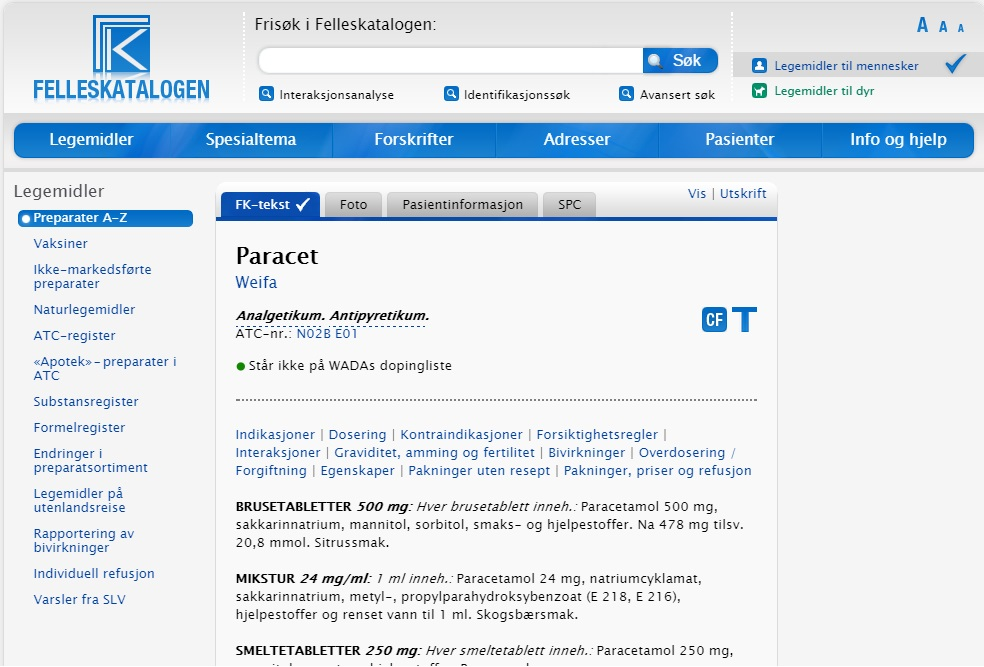
\includegraphics[width=1\textwidth]{fig/dagens/paracetFelleskatalog.jpg}
  \caption{Skjermbilde som viser informasjon om Paracet i Felleskatalogen på internett. Dato: 30.10.2014}
\label{fig:felleskatalogen}
\end{figure}


\subsection{Legemiddelhåndboken}
Legemiddelhåndboken (Norsk legemiddelhåndbok for helsepersonell) er et terapiorientert oppslagsverk for legemidler som behandlingsalternativ. Legemiddelhåndboken er en viktig kilde til leverandørnøytral informasjon om indikasjoner, bruk, virkninger og bivirkninger av legemidler. 
 
Legemiddelhåndboken er rettet mot leger. Det er derfor lagt særlig vekt på å omtale tilstander hvor legemidler har en viktig plass i behandlingen.
 
Legemiddelhåndboken er delt i fire hovedavsnitt:
\begin{itemize}
    \item en del om sykdommer
    \item en del om legemidler
    \item en generell del som omfatter ulike behandlingssituasjoner og veiledning ved legemiddelbruk
    \item en registerdel med blant annet stikkord og adresseregister
\end{itemize}

\acrshort{start}\footnote{Les mer om START her: \url{http://legemiddelhandboka.no/Generelle/311103}}, \acrshort{stopp}\footnote{Les mer om STOPP her: \url{http://legemiddelhandboka.no/Generelle/315753}} og \acrshort{norgep}\footnote{Les mer om NorGep her: \url{http://legemiddelhandboka.no/Generelle/311393}} er tatt med i legemiddelhåndboken, jf. delkapittel~\ref{subsec:legemiddelgjennomgang}.

Norsk legemiddelhåndbok er tilgjengelig på flere format: den er tilgjengelig på internett \footnote{Legemiddelhåndboken på nett finner du her: \url{www.legemiddelhandboka.no}}, den kan lastes ned lokalt til PC og den er tilgjengelig som en applikasjon til smarttelefoner. Figur~\ref{fig:legemiddelhandbok} viser et skjermbilde fra legemiddelhåndboken på nett.

\begin{figure}[H]
  \centering
    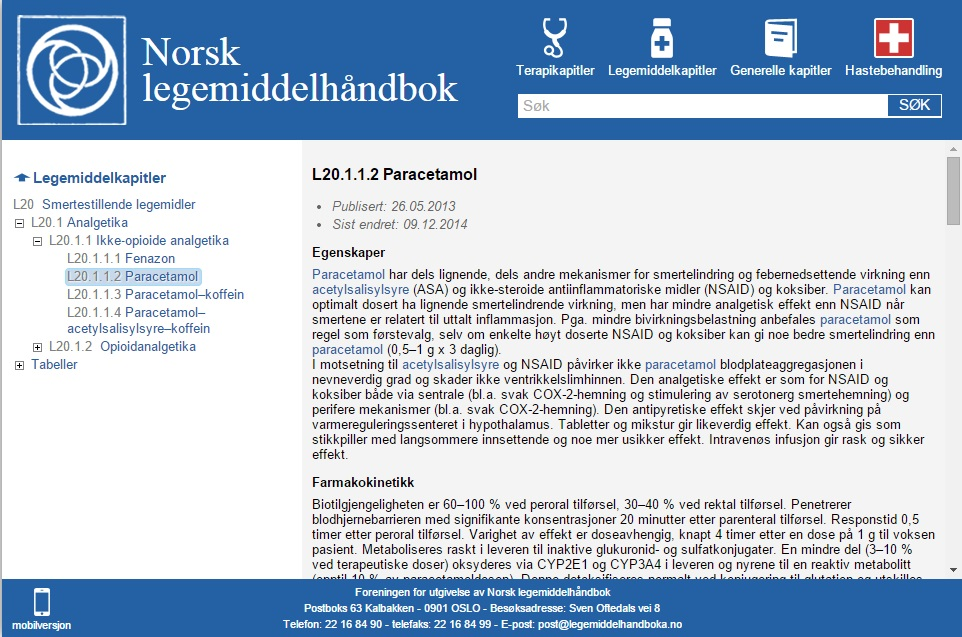
\includegraphics[width=1\textwidth]{fig/dagens/paracetLegemiddelhandbok.jpg}
  \caption{Skjermbilde som viser informasjon om Paracetamol i legemiddelhåndboken på internett. Dato: 30.10.2014}
\label{fig:legemiddelhandbok}
\end{figure}


\subsection{FEST}
\acrfull{fest} er en database utviklet av Legemiddelverket. Databasen inneholder informasjon om alle legemidler som kan kjøpes på resept i Norge. Målet med \acrshort{fest} er å fremme trygg legemiddelbruk, og gi oppdatert og samstilt informasjon til leger, apoteker og bandasjister. \acrshort{fest} presenterer data i \acrshort{xml}-format\footnote{XML: er et markeringsspråk som definerer et sett av regler for koding av dokumenter til et format som både kan leses av mennesker og maskiner.} og en er viktig del av datagrunnlaget for andre systemer, blant annet en forutsetninger for innføring av e-Resept \citep{omFEST}. 

\subsection{Interaksjoner.no}
Interaksjoner.no er et verktøy for å søke etter legemiddelinteraksjoner ved å bruke norske handelsnavn. Interaksjoner.no er basert på \acrshort{fest}, og det er Legemiddelverket som er ansvarlig for innholdet i databasen. 

Motivasjonen for å utvikle verktøyet er at manuelle oppslag på mulige interaksjoner for hvert enkelt legemiddel er tidkrevende, og at andre systemer for å sjekke interaksjoner ikke gjenkjenner norske handelsnavn \citep{OmInteraksjonerdotno}. 

Figur~\ref{fig:int} viser et skjermbilde fra interaksjoner.no med resultater ved søk på Albyl-E. I listen over interaksjoner er det brukt \acrshort{atc}-koder istedenfor norske handelsnavn på legemidler. Dette kan gjøre det vanskelig for pasienter å forstå hvilke legemidler som er delaktig i interaksjonene.

\begin{figure}[H]
  \centering
    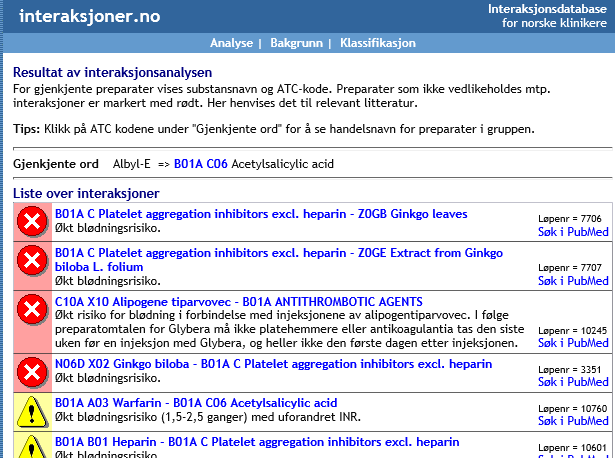
\includegraphics[width=1\textwidth]{fig/dagens/interaksjoner.png}
  \caption{Skjermbilde fra \url{www.interaksjoner.no} som viser resultatet av søk på Albyl-E. Dato: 09.11.2014}
\label{fig:int}
\end{figure}

\subsection{RELIS}
\acrshort{relis} (\acrlong{relis}) er en offentlig finansiert informasjonstjeneste som skal gi produsentuavhengig legemiddelinformasjon til helsepersonell. Hensikten er at \acrshort{relis} skal bidra til forsvarlig, rasjonell og riktig bruk av legemidler.
 
Ved universitetsykehus i alle de fire helseregionene er det etablert \acrshort{relis}-sentre. Alle sentrene er knyttet til de klinisk farmakologiske fagmiljøene ved universitetssykehusene, og har et bredt samarbeid med helsepersonell i regionene. På \url{www.relis.no/database} har \acrshort{relis} en spørsmål-svar tjeneste, se figur~\ref{fig:int}. Tjenesten er beregnet på helsepersonell, og er ment å være til hjelp med legemiddelspørsmål.

\begin{figure}[H]
  \centering
    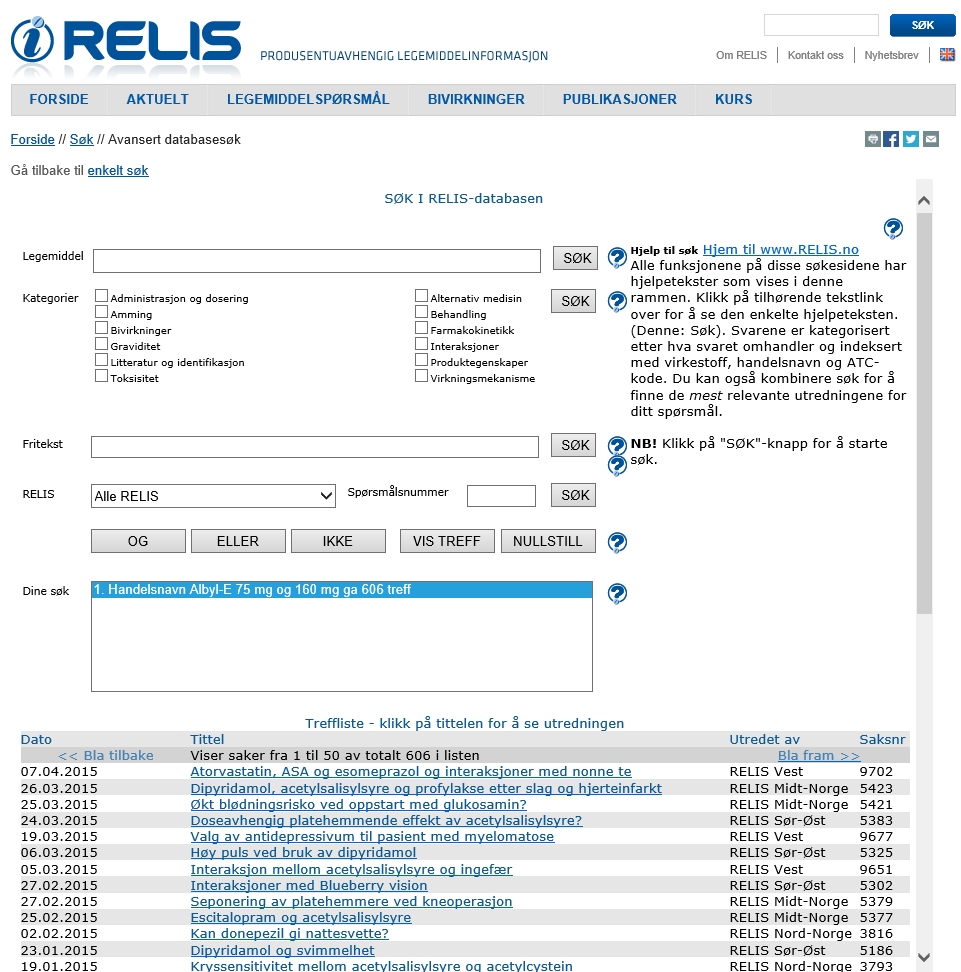
\includegraphics[width=1\textwidth]{fig/dagens/relis.png}
  \caption{Skjermbilde som viser \url{www.relis.no/database} ved søk på Albyl-E.  Dato: 15.02.2015}
\label{fig:relis}
\end{figure}

\acrshort{relis} har ansvaret for bivirkningsovervåkningen på oppdrag fra Statens Legemiddelverk. De mottar bivirkningsmeldinger, vurderer hendelsesforløp og årsakssammenheng og kommentarer i skriftlig tilbakemelding til melder. Bivirkningsrapportene blir registrert i en nasjonal bivirkningsdatabase.


\section{Pasientkontrollerte systemer}
Her presenteres pasientkontrollerte systemer som er utviklet av store internasjonale selskaper, men som er lite tatt i bruk i Norge. 

\subsection{Google Health}
Google Health var en personlig helsejournal laget av Google. Systemet fungerte ved at brukere la inn helseinformasjon manuelt eller ved dataoverføring fra helsetjenesten. Når informasjon var lagt inn i systemet kunne Google Health vise brukeren en personlig journal og vise mulige interaksjoner mellom legemidler. I 2011 annonserte Google at Google Health skulle legges ned. Figur~\ref{fig:googleHealth} viser et skjermbilde av hvordan Google health så ut da det eksisterte. 

\subsection{Microsoft HealthVault}
Microsoft HealthVault er en skybasert plattform som skal lagre og vedlikeholde helse- og fitnessinformasjon. Systemet fungerer som en egenopprettet journal hvor brukeren styrer innhold og tilgang. Opplysningene kan legges inn manuelt av brukerne, eller automatisk fra utstyr som kan kobles opp mot HealthVault. Dette kan være opplysninger om legemidler, vaksinasjoner, vekt osv. 

Figur~\ref{fig:HealthVault} viser et skjermbilde av HealthVault-profilen til Kåre. Det er lagt inn informasjon om Kåre sine legemidler og lidelser som fritekst. HealthVault er ikke i stand til å gjøre noe resonnering basert på informasjonen som er lagt inn, og Kåre kan ikke få informasjon om mulige interaksjoner eller bivirkninger. 


\subsection{Dossia}
I 2006 ble Dossia grunnlagt som et samarbeidsprosjekt mellom flere arbeidsgivere. Målet var å gi sine ansatte en helsejournal. Dossia er en personlig helsejournaltjeneste. Den gjør det mulig for pasienter å samle kopier av sine egne helsedata fra ulike steder, for å lage en personlig og elektroniske helsejournal.

\subsection{Indivo}
Indivo er en helsejournalplattform laget av \acrfull{chip}. Den fokuserer på å gi brukere kontroll over egen helsejournal. Det er en plattform som muliggjør utvikling av personlige helseapplikasjoner hvor pasienter kan se og legge inn merknader til informasjonen. Indivio har blitt brukt i Microsoft sitt prosjekt HealthVault, har inspirerte arkitekturen til Google Health og har blitt brukt i Dossias helsejournal.

\begin{figure}[H]
  \centering
    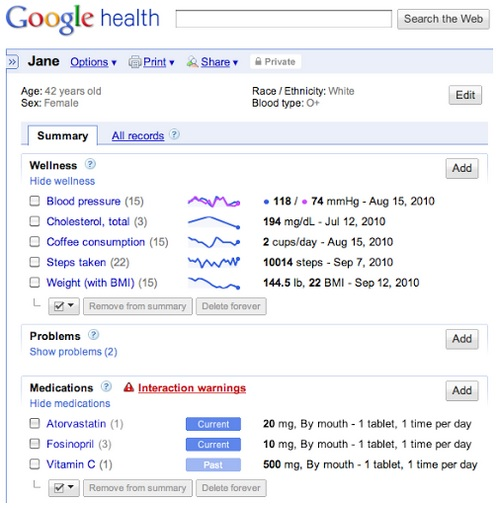
\includegraphics[width=1\textwidth]{fig/dagens/GoogleHealth.jpg}
  \caption{Skjermbilde som viser hvordan GoogleHealth så ut. Hentet fra: \url{http://googleblog.blogspot.no/2010/09/google-health-update.html}}
\label{fig:googleHealth}
\end{figure}

\begin{figure}[H]
  \centering
    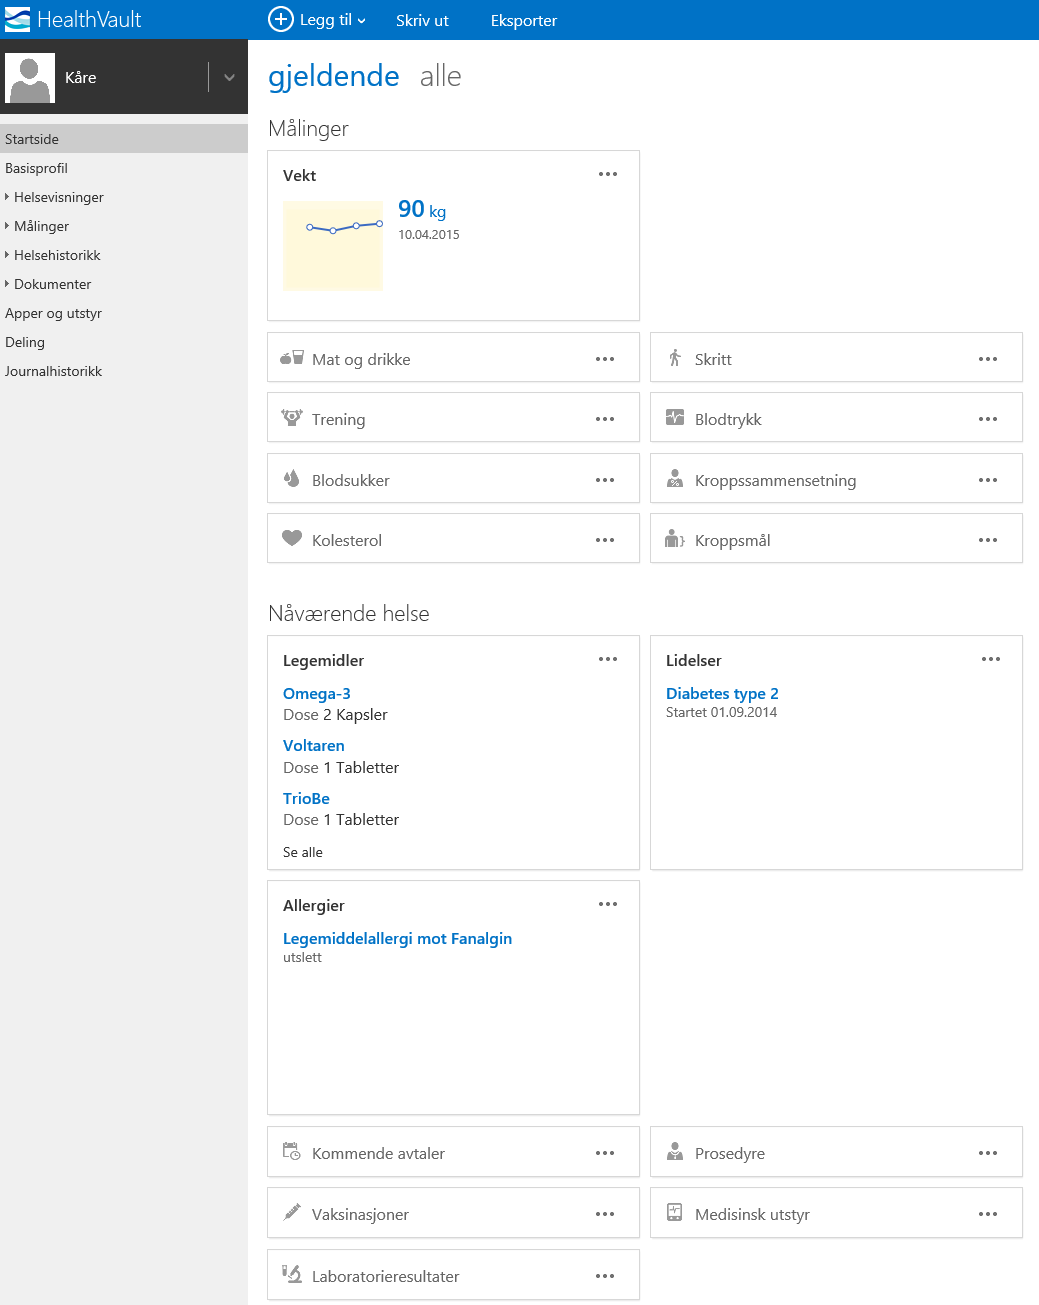
\includegraphics[width=1\textwidth]{fig/dagens/HealthVault.png}
  \caption{Skjermbilde fra HealthVault for Kåre 77 år. Dato 10.04.2015}
\label{fig:HealthVault}
\end{figure}


\section{Personvern} \label{sec:sikkerhet}
Økt bruk av elektronisk behandling av informasjon og personopplysninger skaper mange muligheter, men det medfører også utfordringer for personvern. Elektronisk behandling av opplysninger om pasienter medfører at opplysningene lett kan bli tilgjengelig både internt i helsevesenet og eksternt for pasienter og pårørende. Det er viktig å passe på at uvedkommende ikke får tilgang til opplysninger som er lagret elektronisk. I det følgende blir viktige lover og regler som skal sikte at personvernet er ivaretatt av legemiddelinformasjonskilder presentert kort.


\subsection{Lov om medisinsk utstyr}
Det norske lovverket er i samsvar med \acrshort{eu}s bestemmelser vedrørende medisinsk utstyr (medical devices), jf. direktiv 2007/47/EC. Lov om medisinsk utstyr regulerer “produksjon, markedsføring, omsetning og bruk av medisinsk utstyr”, jf. lov om medisinsk utstyr § 1. Formålet med loven er å forhindre skader og å sikre at medisinsk utstyr blir brukt på forsvarlig måte, jf. lov om medisinsk utstyr § 2.

Det er gitt detaljerte regler om merking av medisinsk utstyr, og om hvordan produsenter skal gå frem for å sikre og dokumentere at utstyret fyller de tekniske krav som er satt. Utstyr som er fremstilt i samsvar med regelverket, skal \acrshort{ce}-merkes\footnote{CE-merke er et godkjenningsmerke innenfor EØS-området}, jf. lov om medisinsk utstyr § 5 og forskrift om medisinsk utstyr § 2-4.

For å falle under lovens definisjon av medisinsk utstyr må det være “ment å skulle brukes på mennesker”, jf. lov om medisinsk utstyr § 3 første ledd. Det er noe uklart hvorvidt kilder til personlige legemiddelinformasjon faller under ordlyden av dette. Lov om medisinsk utstyr § 3 fjerde ledd, angir at det i tvilstilfeller er departementet som avgjør om noe er å regne som medisinsk utstyr.
 
Generelt sett skal sosial- og helsedirektoratet føre tilsyn med at regelverket om medisinsk utstyr overholdes. Direktoratet for samfunnssikkerhet og beredskap har også en tilsynsrolle når det gjelder elektronisk medisinutstyr.

\subsection{Personopplysningsloven og helseregisterloven}
I Norge stiller Personvern- og helselovgivningen krav til informasjonssikkerhet\footnote{Informasjonssikkerhet: samlebetegnelse for krav til påliteligheten og sikkerheten som knyttes til informasjon.}. Aktuelle tilsynsmyndigheter (Datatilsynet og Helsetilsynet) har ansvar for å kontrollere etterlevelse av gjeldende regelverk.
 
Personopplysningsloven gir grunnleggende regler innen personvern og informasjonssikkerhet. I Helseregisterloven finnes regler om hvordan virksomheter skal behandle pasienters helseopplysninger. Kravene i helseregisterloven er harmonisert med de generelle kravene som gjelder ved behandling av personopplysninger etter personopplysningsloven. Dette er fordi begge lovene bygger på EUs personverndirektiv (95/46/EF), og fordi det ikke er ønskelig med utvikling av forskjellige sikkerhetsnivåer i forskjellige samfunnssektorer \citep{kommentarutgaveHelseregisterloven}.
 
Formålet med helseregisterloven er å bidra til at helseopplysninger kan samles inn og brukes til helsefremmende formål, uten å krenke personvernet, jf. helseregisterloven § 1. Opplysninger  registrert om en pasient i et digitalt system er etter loven regnet som «helseopplysninger», jf. helseregisterloven § 2 bokstav a. Personlige systemer for legemiddelinformasjon må derfor følge bestemmelsene i helseregisterloven om behandlingen av helseopplysninger.

\subsection{Normen}
Sosial- og helsedirektoratets tok initiativ til at helsesektoren skulle utarbeide sin egen norm for informasjonssikkerhet. Dette resulterte i norm for informasjonssikkerhet i helse-, omsorgs- og sosialsektoren (Normen). Det er en samling retningslinjer og krav som skal bidra til “tilfredsstillende” informasjonssikkerhet hos virksomheter i sektoren. Normen gjelder for alle virksomheter som ved avtale har forpliktet seg til å følge den \citep{OmNormen}.
